\section[Analysis of shunted piezoelectric patches]{Shunted piezoelectric patches}

\begin{frame}{Piezoelectric patches sensitivity to $RLC_N$ shunting circuit}

    \begin{columns}[c, onlytextwidth]

        \begin{column}{0.3\textwidth}

            \begin{figure}[H]

                \centering

                \begin{tikzpicture}[european voltages]

                    % Upper and lower horizontal lines
                    \draw (0,0) to [short] ++(2,0);
                    \draw (0,-4.5) to [short] ++(2,0);

                    % Piezo
                    \draw (0,0) to [C, l=$C_p$, o-o] ++(0,-4.5);

                    % Shunt
                    \draw (2,0)
                    to [R, l=$R$, o-] ++(0,-2)
                    to [L, l=$L$] ++(0,-1)
                    to [C, l=$-C_N$, -o] ++(0,-1.5);

                \end{tikzpicture}

                \caption{$RLC_N$ shunting circuit}

            \end{figure}

        \end{column}

        \hfill

        \begin{column}{0.65\textwidth}

            \textbf{The mechanical admittance of piezoelectric patches is influenced by the presence of shunting circuits}:

            \begin{equation}
                \begin{aligned}
                    Y^{SU} & = Y_1^D \left( 1 - \frac{k_{31}^2}{1 + s C_p^S Z^{SU}} \right)                                               \\
                           & = Y_1^D \left( 1 - \frac{k_{31}^2}{1 + C_p^S \left( -\frac{1}{C_N} - \omega^2 L \right) - s C_p^S R} \right)
                \end{aligned}
                \label{eq:Y_SU_RLC_N}
            \end{equation}

            \vspace{9pt}

            Negative capacitance ($-C_N < 0$) are active elements that can be implemented via OP-AMPs.
            As active elements, stability analysis is required:

            \begin{itemize}
                \item Mechanically stable if $Y^{SU} > 0$;
                \item Electrically stable if $C_{tot} > 0$.
            \end{itemize}

        \end{column}

    \end{columns}

    \vspace{9pt}

    A complete sensitivity analysis of $Y^{SU}(Z^{SU})$ is shown in the next slides.

\end{frame}



\begin{frame}{Short vs. Open circuit case}

    \begin{figure}[H]
        \centering
        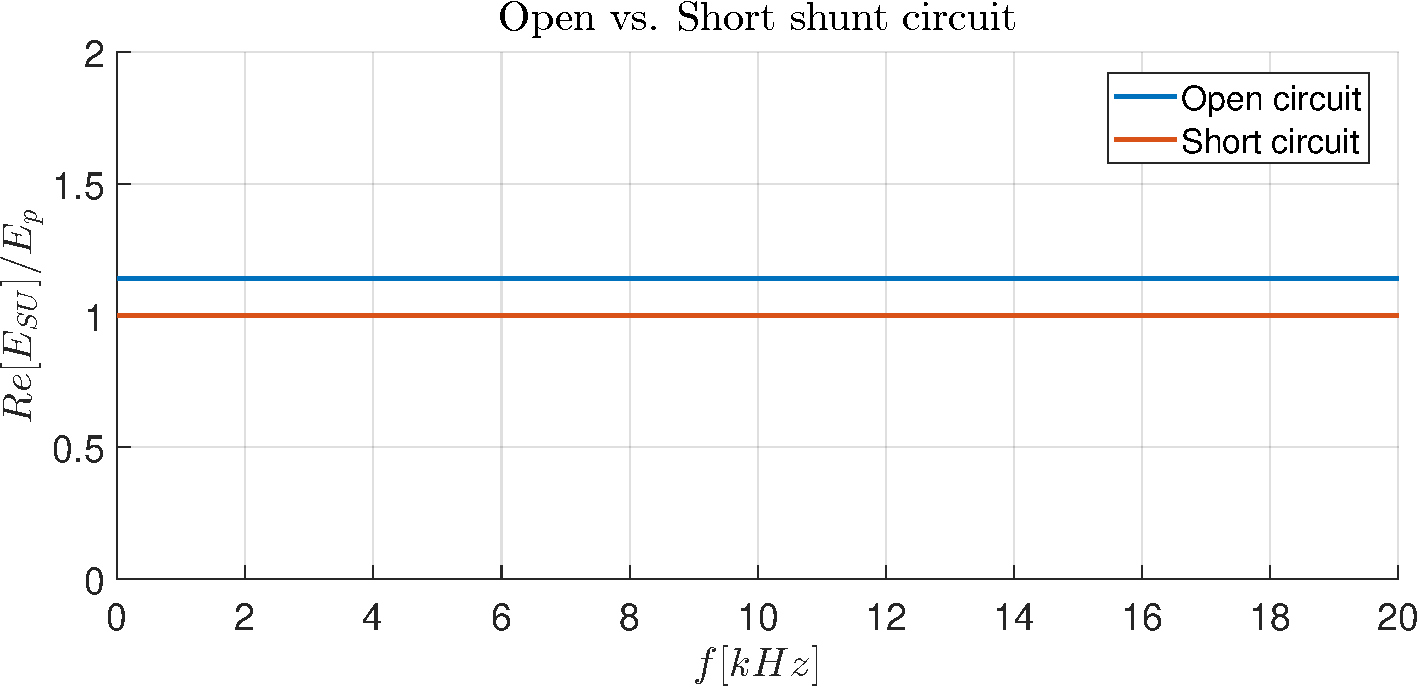
\includegraphics[width=0.7\textwidth]{./img/MATLAB/Y_SU_Open vs Short circuit.pdf}
        \caption{Analysis of $Y^{SU}$ for the open and short circuit case.}
    \end{figure}

    As predicted by Equation \ref{eq:Y_SU_RLC_N}, the piezoelectric patches' mechanical admittance in case of open circuit is greater than in case of short circuit.
    This causes a stiffer substrate and indeed a shift of the band-gap towards higher frequencies.

    \begin{equation}
        Y_1^D > Y_1^E = Y_1^D (1 - k_{31}^2)
    \end{equation}

\end{frame}



\begin{frame}{Short vs. Open circuit case}


    \only<1-2>{

        \begin{figure}[H]
            \centering
            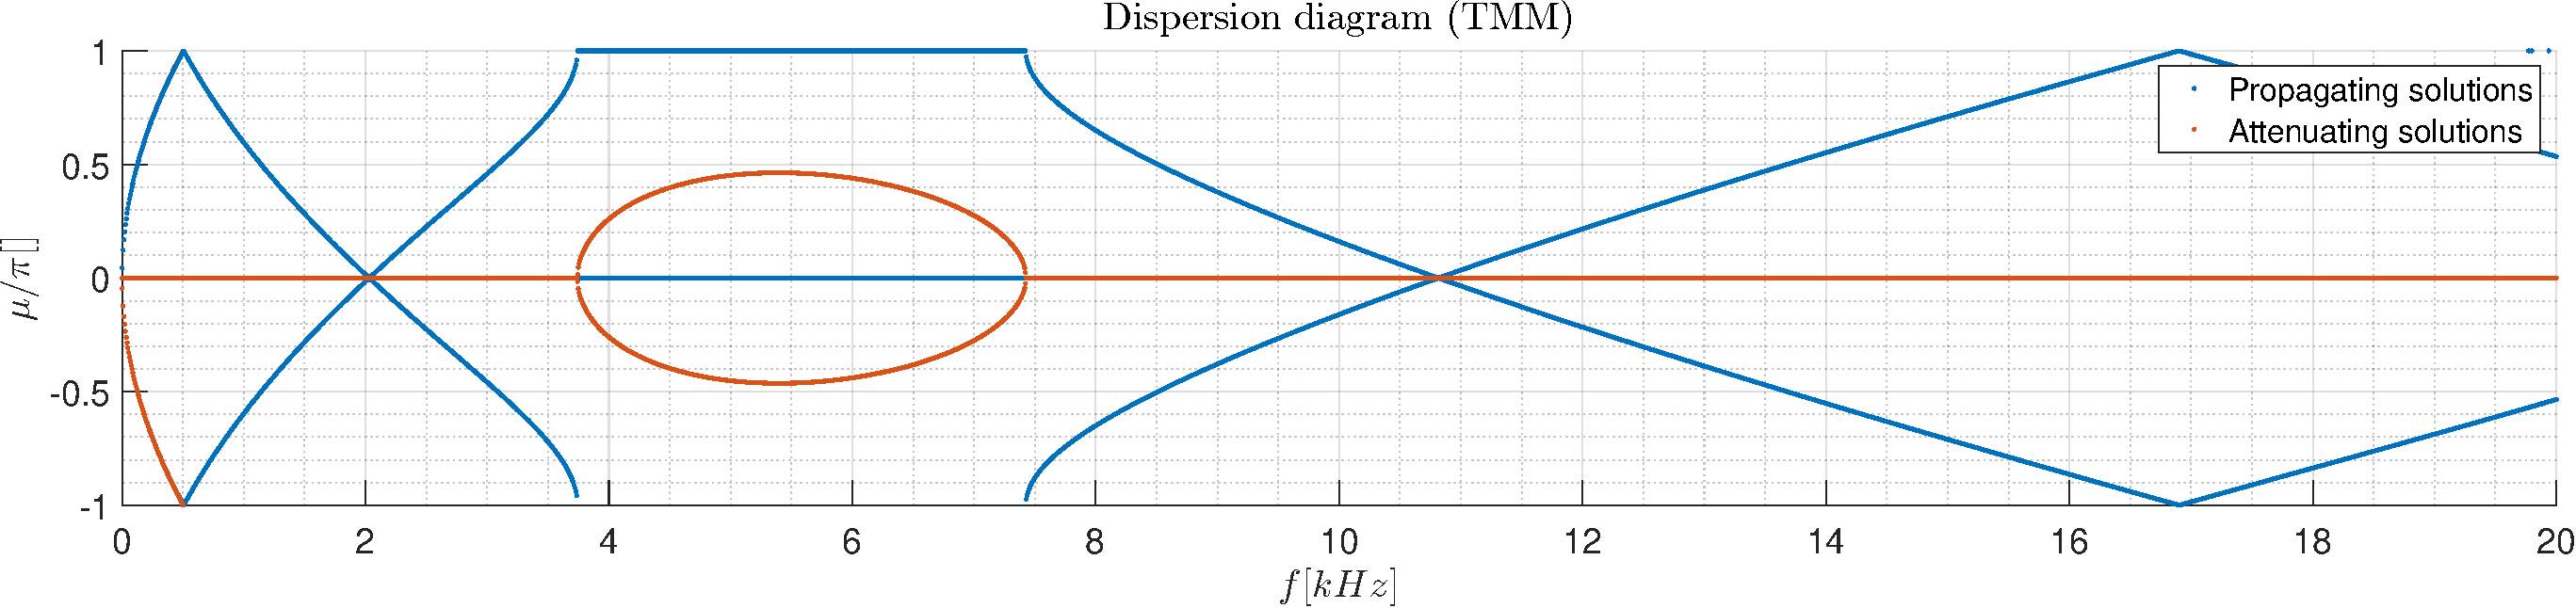
\includegraphics[width=\textwidth]{./img/MATLAB/TMM_ON-ON-ON_OFF_R1000_L0.015_C5e-09.pdf}
            \caption{Short circuit case.}
        \end{figure}

    }

    \only<2->{

        \begin{figure}[H]
            \centering
            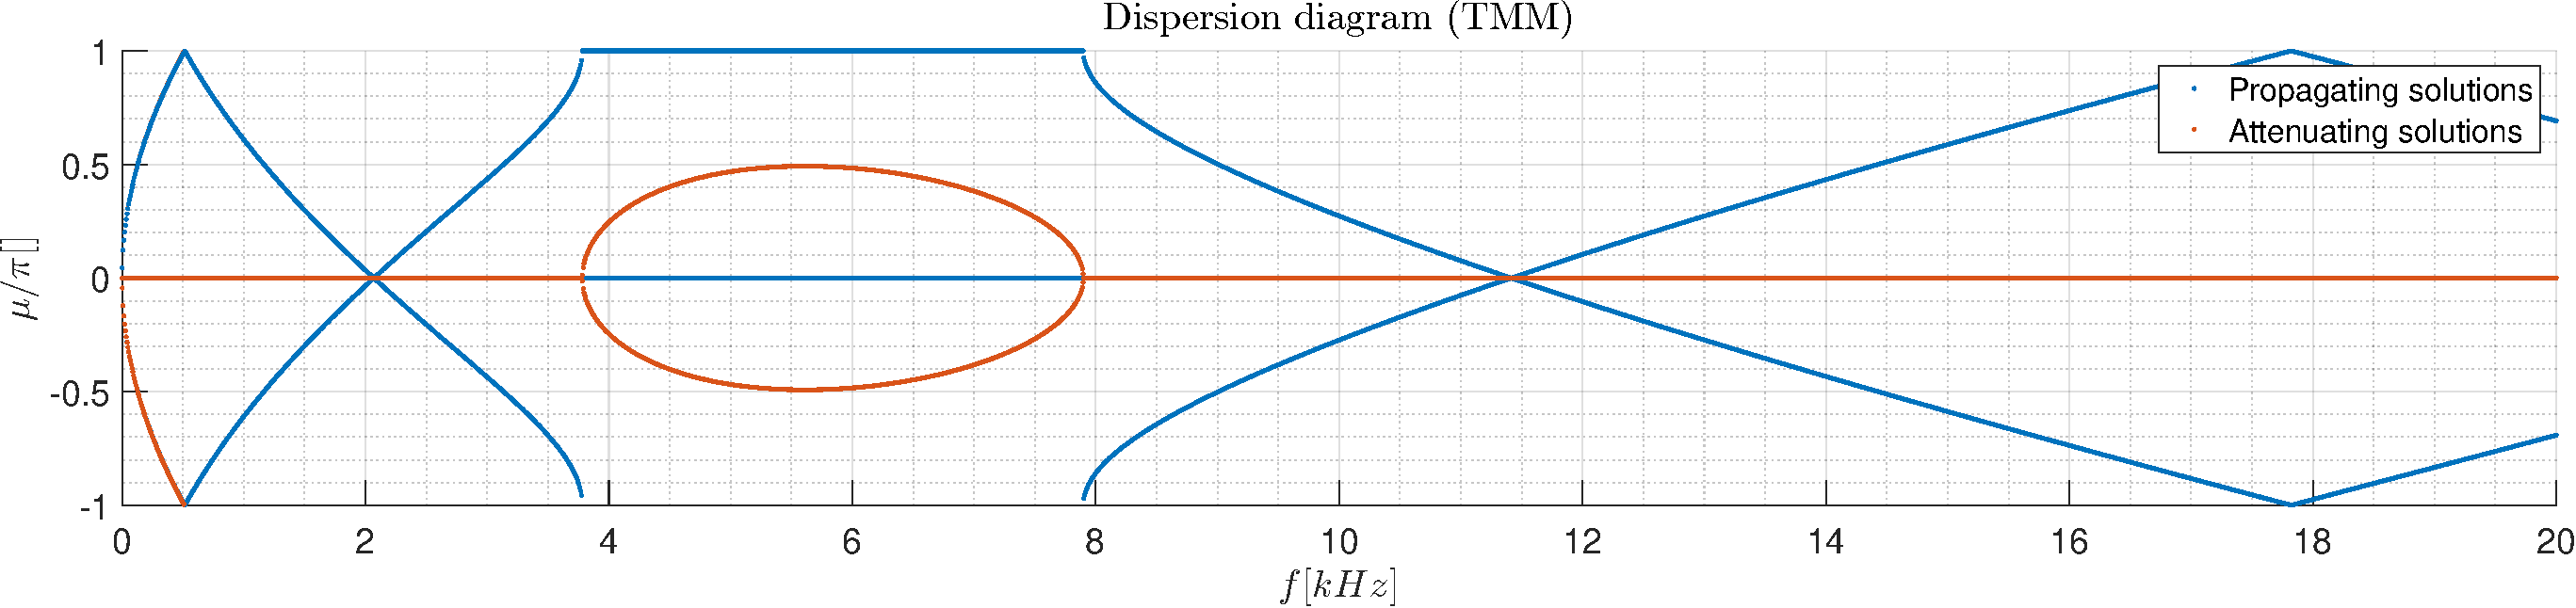
\includegraphics[width=\textwidth]{./img/MATLAB/TMM_ON-ON-ON_+inf_R1000_L0.015_C5e-09.pdf}
            \caption{Open circuit case.}
        \end{figure}

    }

\end{frame}



\begin{frame}{$L$ shunt circuit}

    \begin{figure}[H]
        \centering
        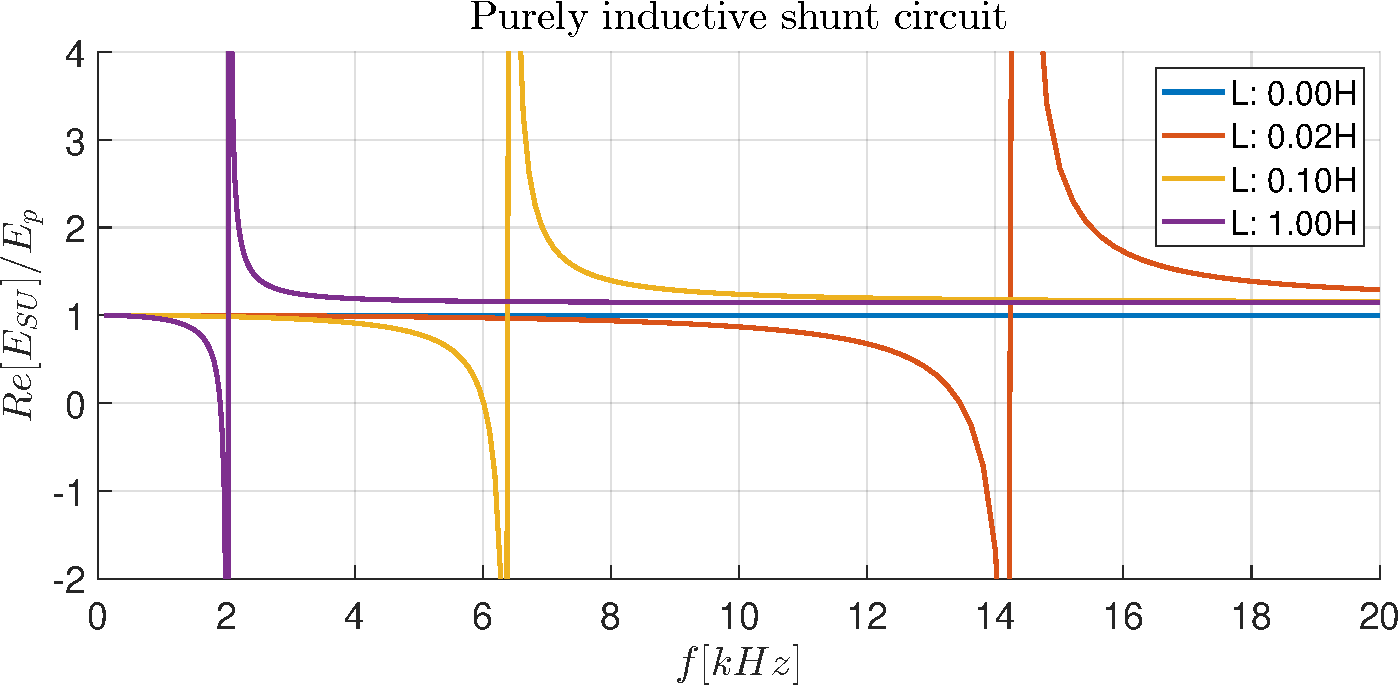
\includegraphics[width=0.7\textwidth]{./img/MATLAB/Y_SU_Purely inductive shunt circuit.pdf}
        \caption{Analysis of $Y^{SU}$ for the purely inductive shunt circuit.}
    \end{figure}

    In case of $L$ shunt circuit, mechanical admittance of the piezoelectric patches is given by:

    \begin{equation}
        Y^{SU} = Y_1^D \left( 1 - \frac{k_{31}^2}{1 -\omega^2 C_p^S L} \right)
    \end{equation}

    Oscillatory behavior is expected around the natural frequency $\omega_n = \frac{1}{\sqrt{C_p^S L}}$.

\end{frame}



\begin{frame}{$L$ shunt circuit}

    \only<1-2>{

        \begin{figure}[H]
            \centering
            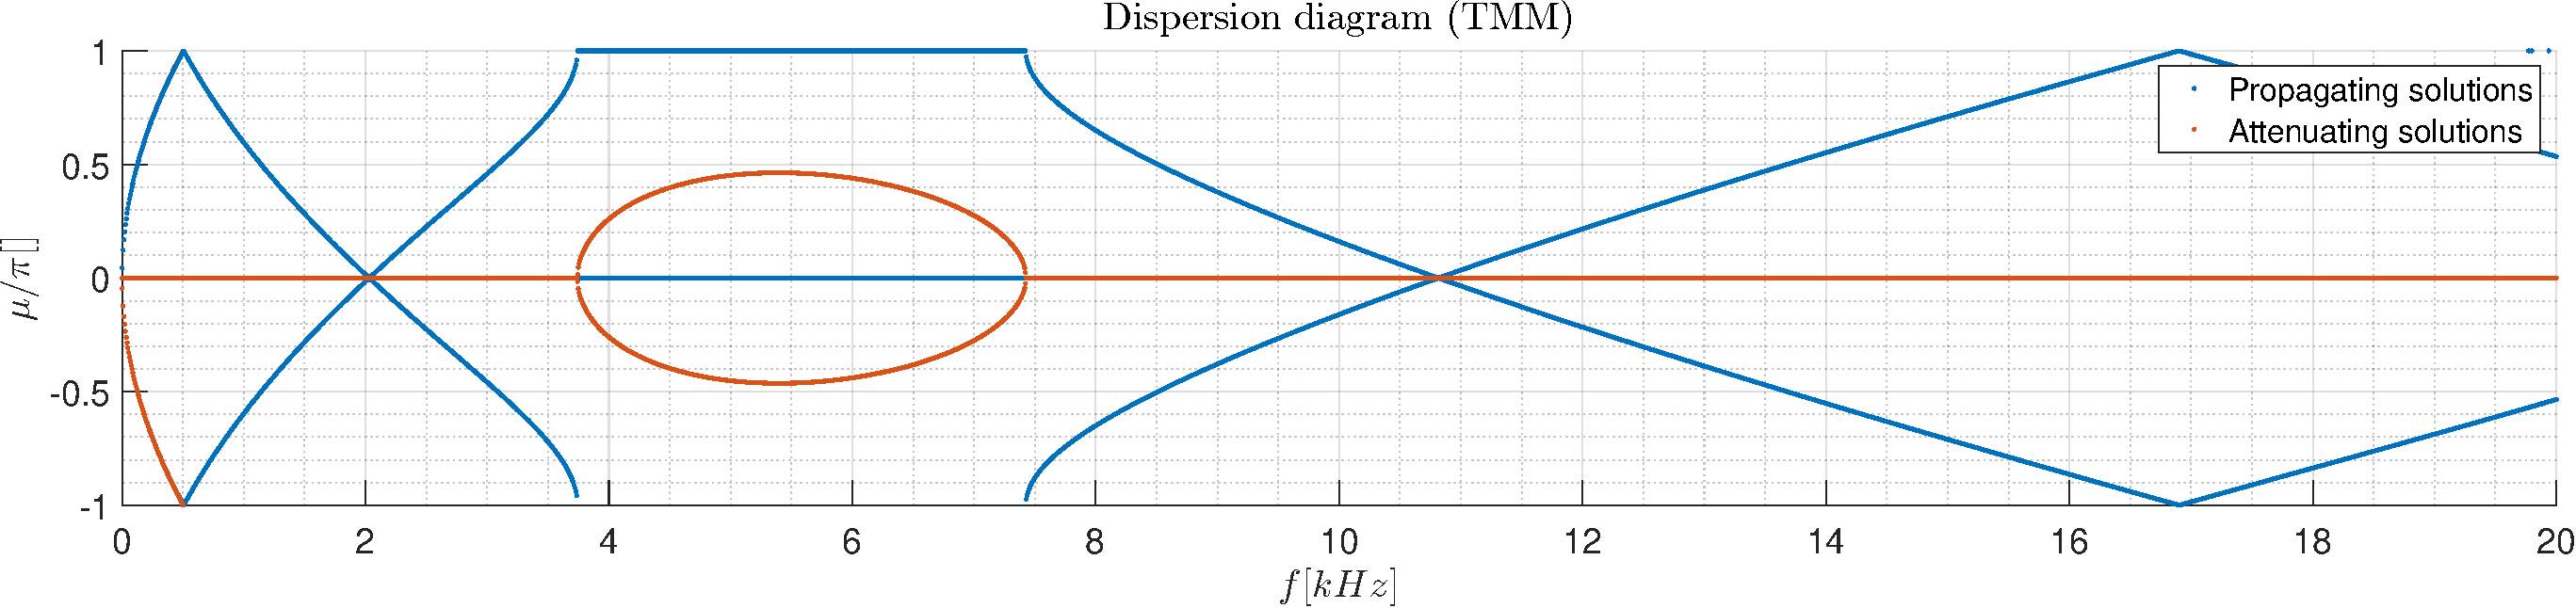
\includegraphics[width=\textwidth]{./img/MATLAB/TMM_ON-ON-ON_RLC_R0_L0_CInf.pdf}
            \caption{RLC shunt circuit with $R = 0 \Omega$, $L = 0 H$, and $C = \infty F$.}
        \end{figure}

    }

    \only<2-3>{

        \begin{figure}[H]
            \centering
            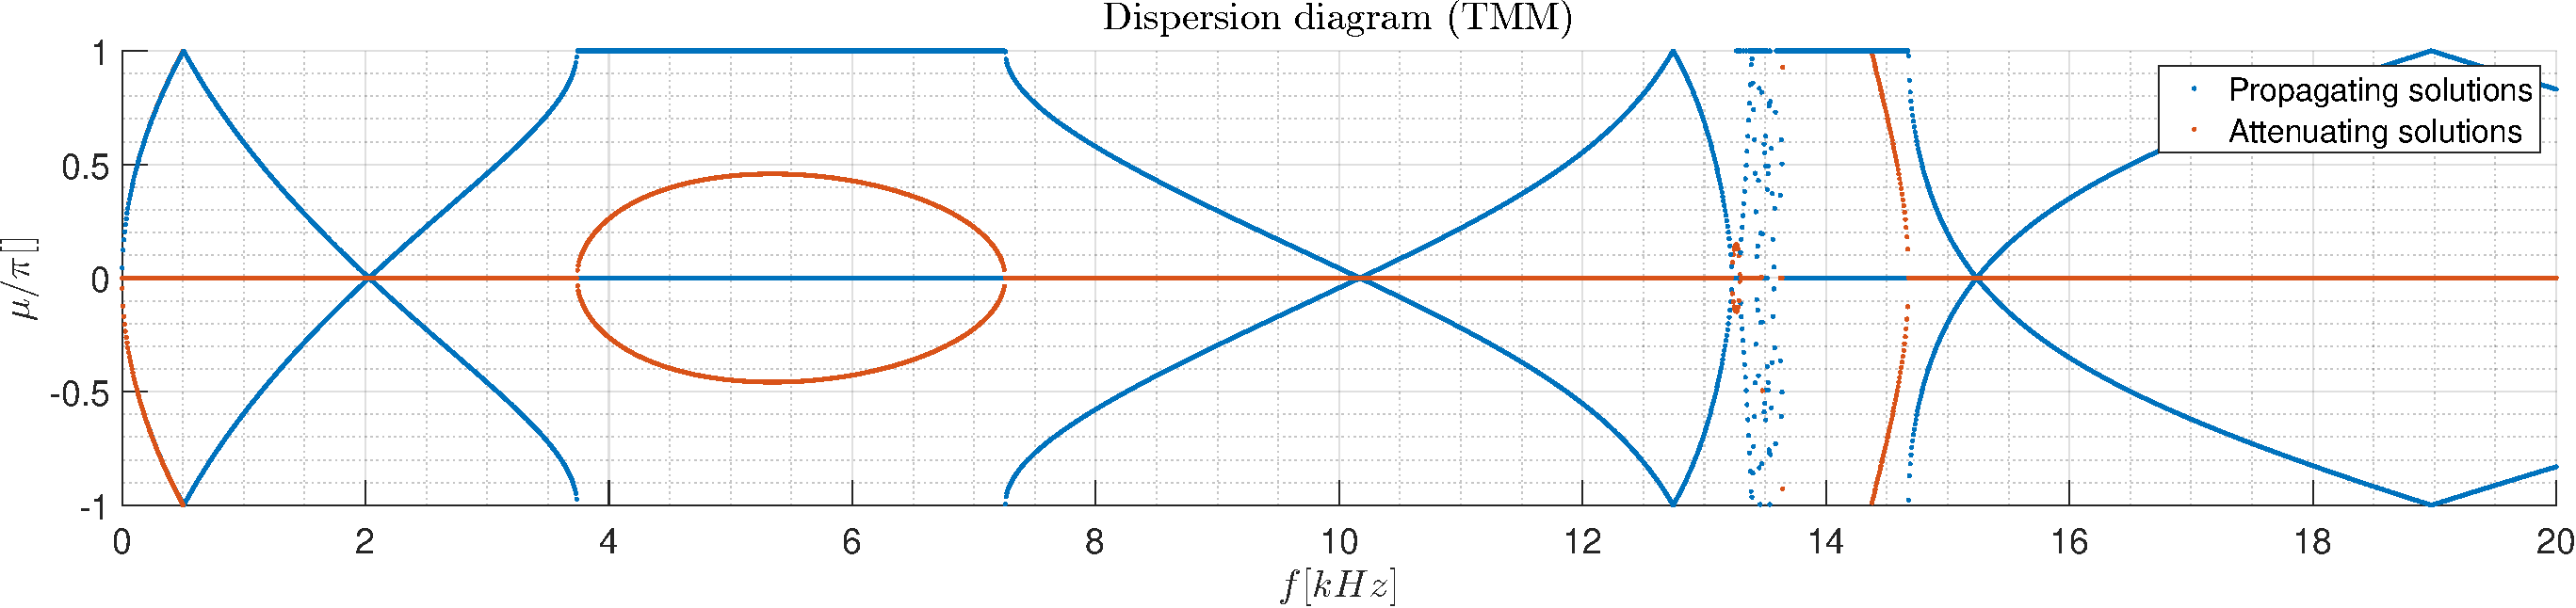
\includegraphics[width=\textwidth]{./img/MATLAB/TMM_ON-ON-ON_RLC_R0_L0.02_CInf.pdf}
            \caption{RLC shunt circuit with $R = 0 \Omega$, $L = 0.02 H$, and $C = \infty F$.}
        \end{figure}

    }

    \only<3-4>{

        \begin{figure}[H]
            \centering
            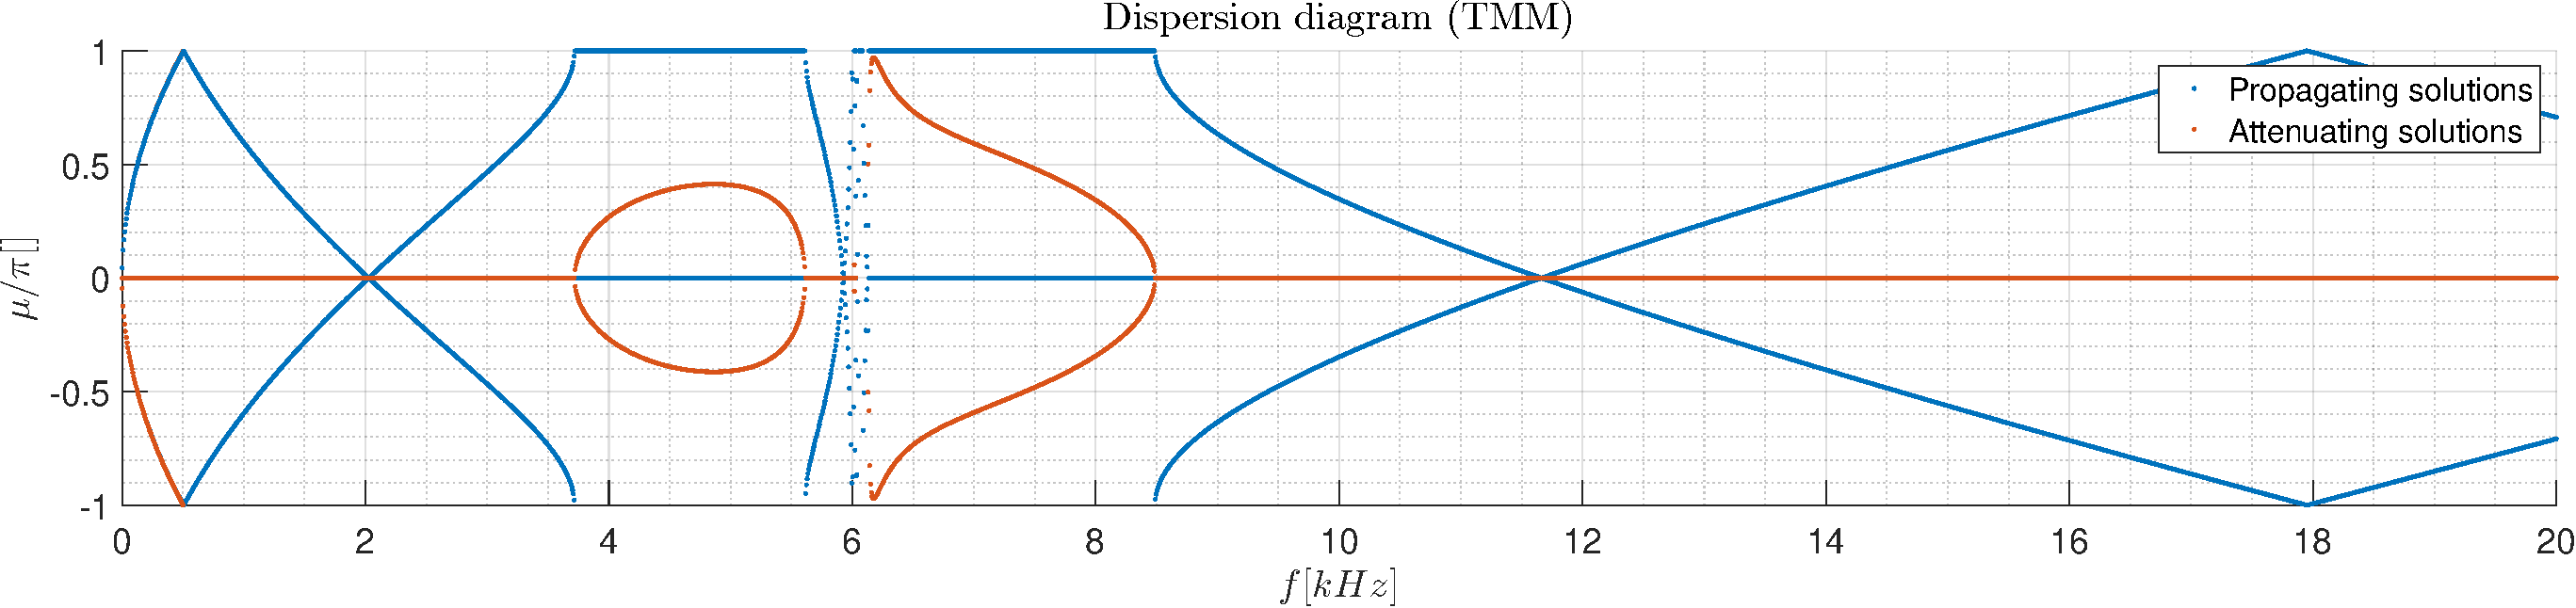
\includegraphics[width=\textwidth]{./img/MATLAB/TMM_ON-ON-ON_RLC_R0_L0.1_CInf.pdf}
            \caption{RLC shunt circuit with $R = 0 \Omega$, $L = 0.10 H$, and $C = \infty F$.}
        \end{figure}

    }

    \only<4->{

        \begin{figure}[H]
            \centering
            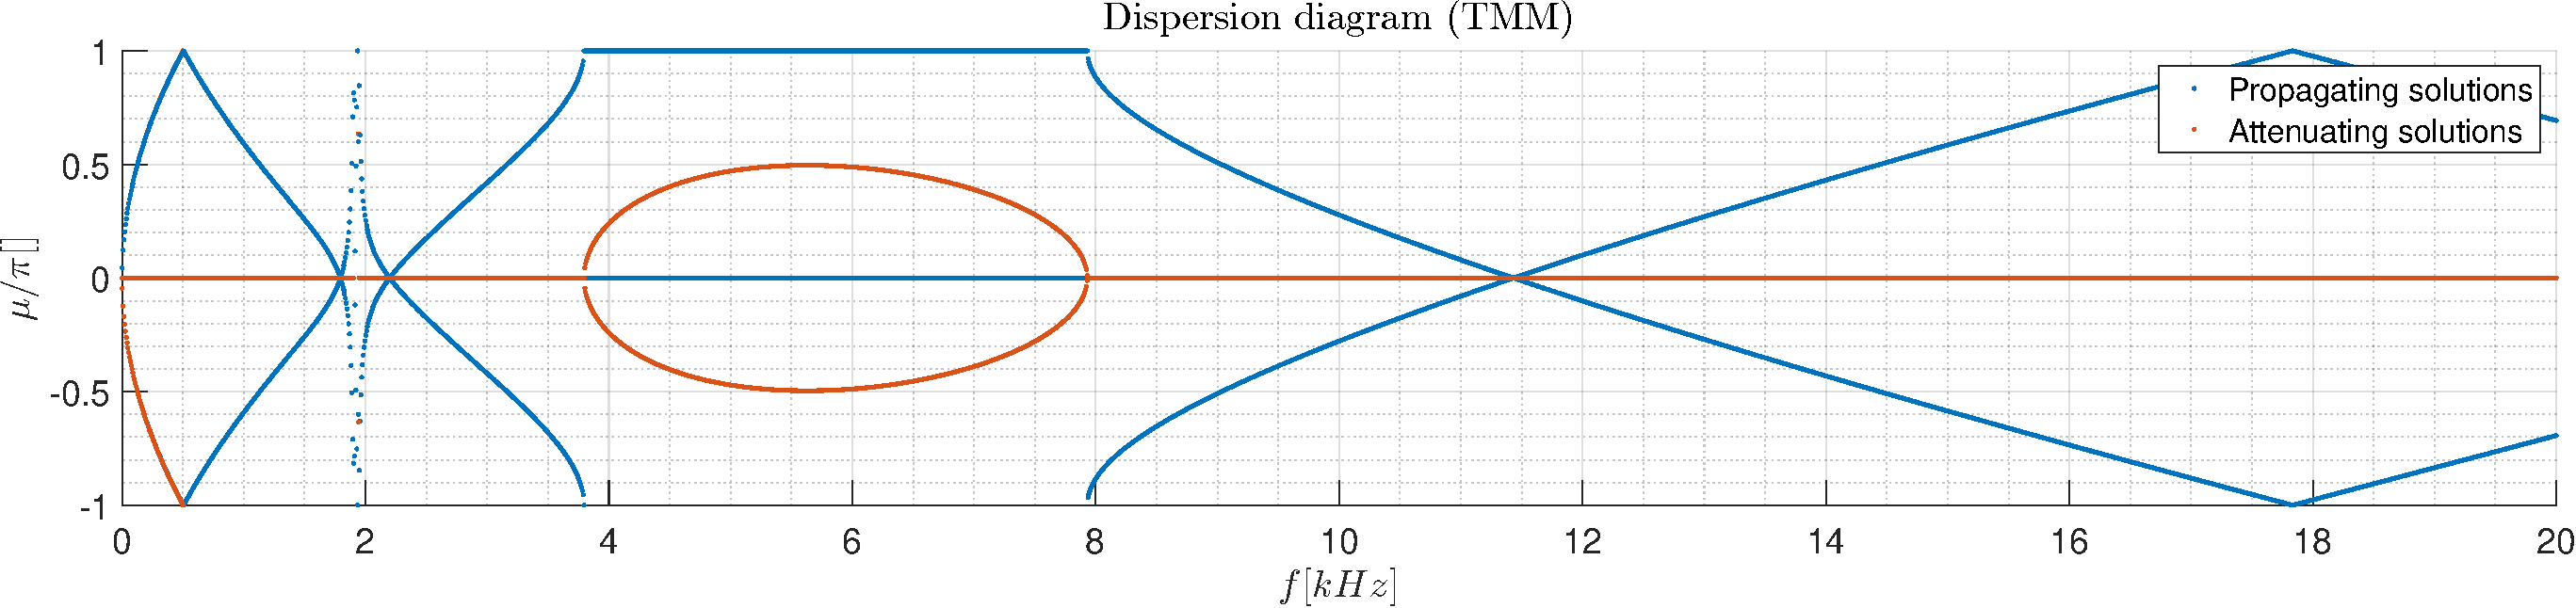
\includegraphics[width=\textwidth]{./img/MATLAB/TMM_ON-ON-ON_RLC_R0_L1_CInf.pdf}
            \caption{RLC shunt circuit with $R = 0 \Omega$, $L = 1 H$, and $C = \infty F$.}
        \end{figure}

    }

\end{frame}



\begin{frame}{$RL$ shunt circuit}

    \begin{figure}[H]
        \centering
        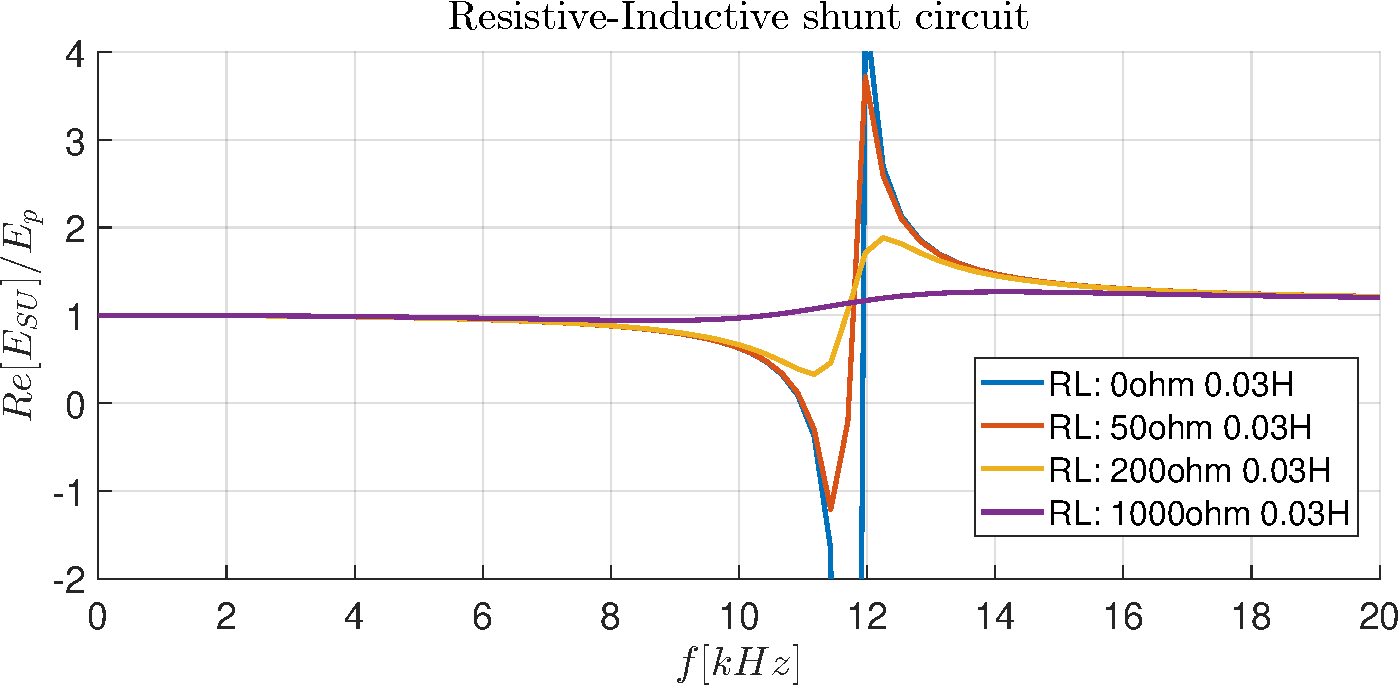
\includegraphics[width=0.6\textwidth]{./img/MATLAB/Y_SU_Resistive-Inductive shunt circuit.pdf}
        \caption{Analysis of $Y^{SU}$ for the resistive-inductive shunt circuit.}
    \end{figure}

    In case of $RL$ shunt circuit, mechanical admittance of the piezoelectric patches is given by:

    \begin{equation}
        Y^{SU} = Y_1^D \left( 1 - \frac{k_{31}^2}{1 -\omega^2 C_p^S L - s C_p^S R} \right)
    \end{equation}

    The resistive element $R$ acts as a damping factor, controlling the width and depth of the band-gap.
    For high values of $R$, the band-gap can be completely suppressed.

\end{frame}


\begin{frame}{$RL$ shunt circuit}


    \only<1-2>{

        \begin{figure}[H]
            \centering
            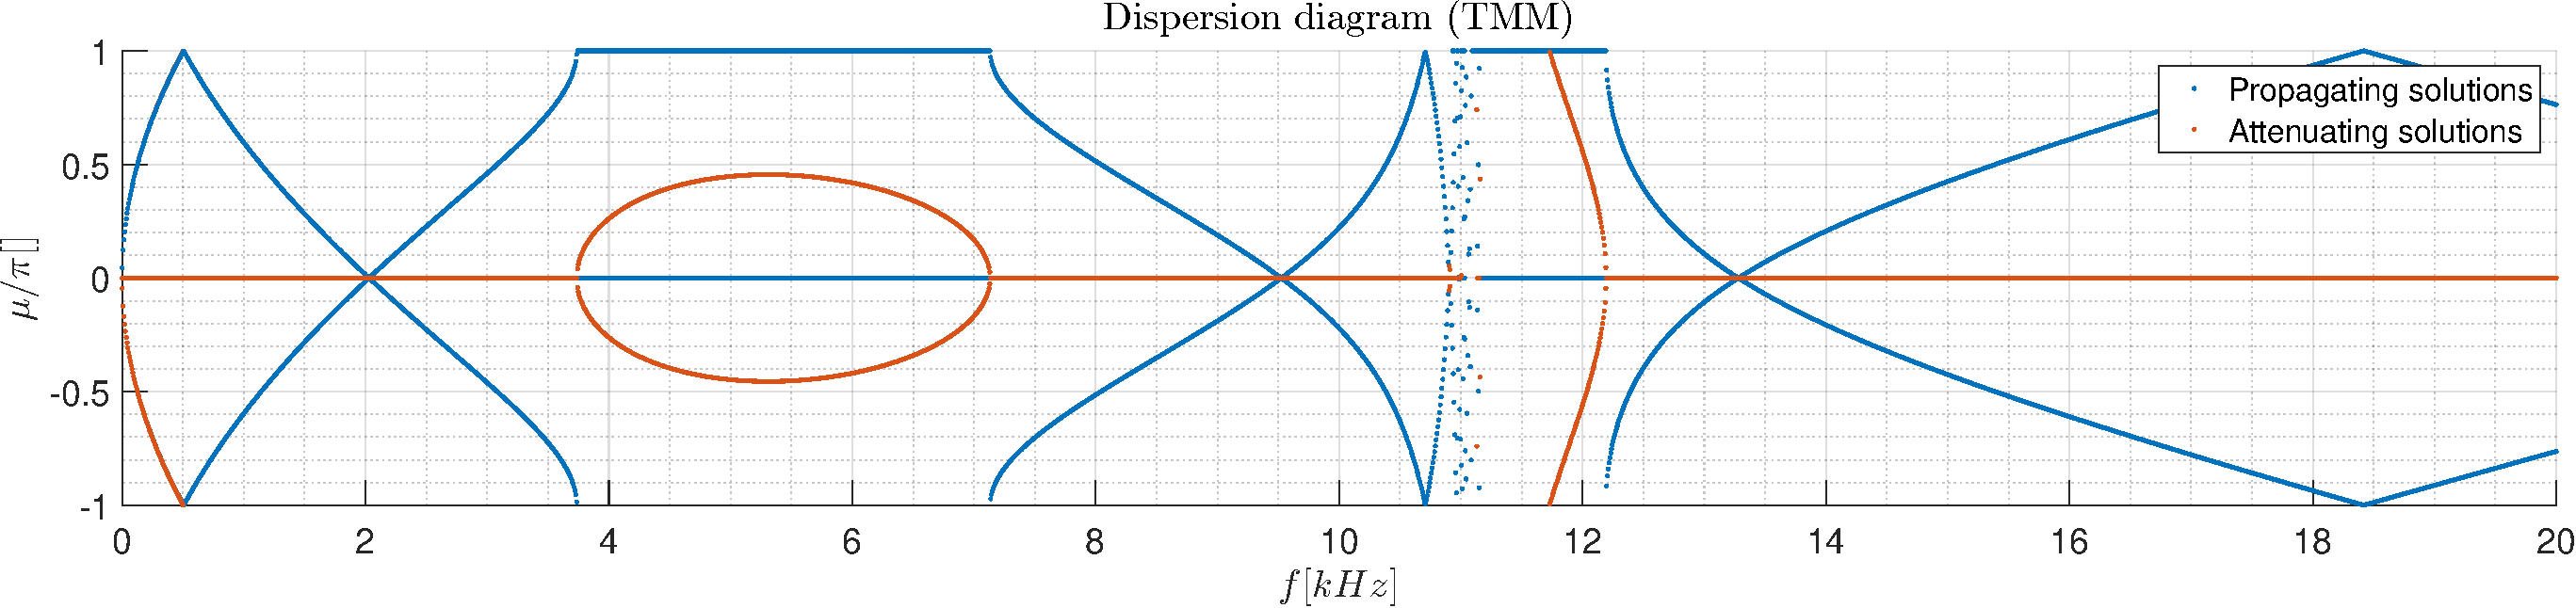
\includegraphics[width=\textwidth]{./img/MATLAB/TMM_ON-ON-ON_RLC_R0_L0.03_CInf.pdf}
            \caption{RLC shunt circuit with $R = 0 \Omega$, $L = 0.03 H$, and $C = \infty F$.}

        \end{figure}

    }

    \only<2-3>{

        \begin{figure}[H]
            \centering
            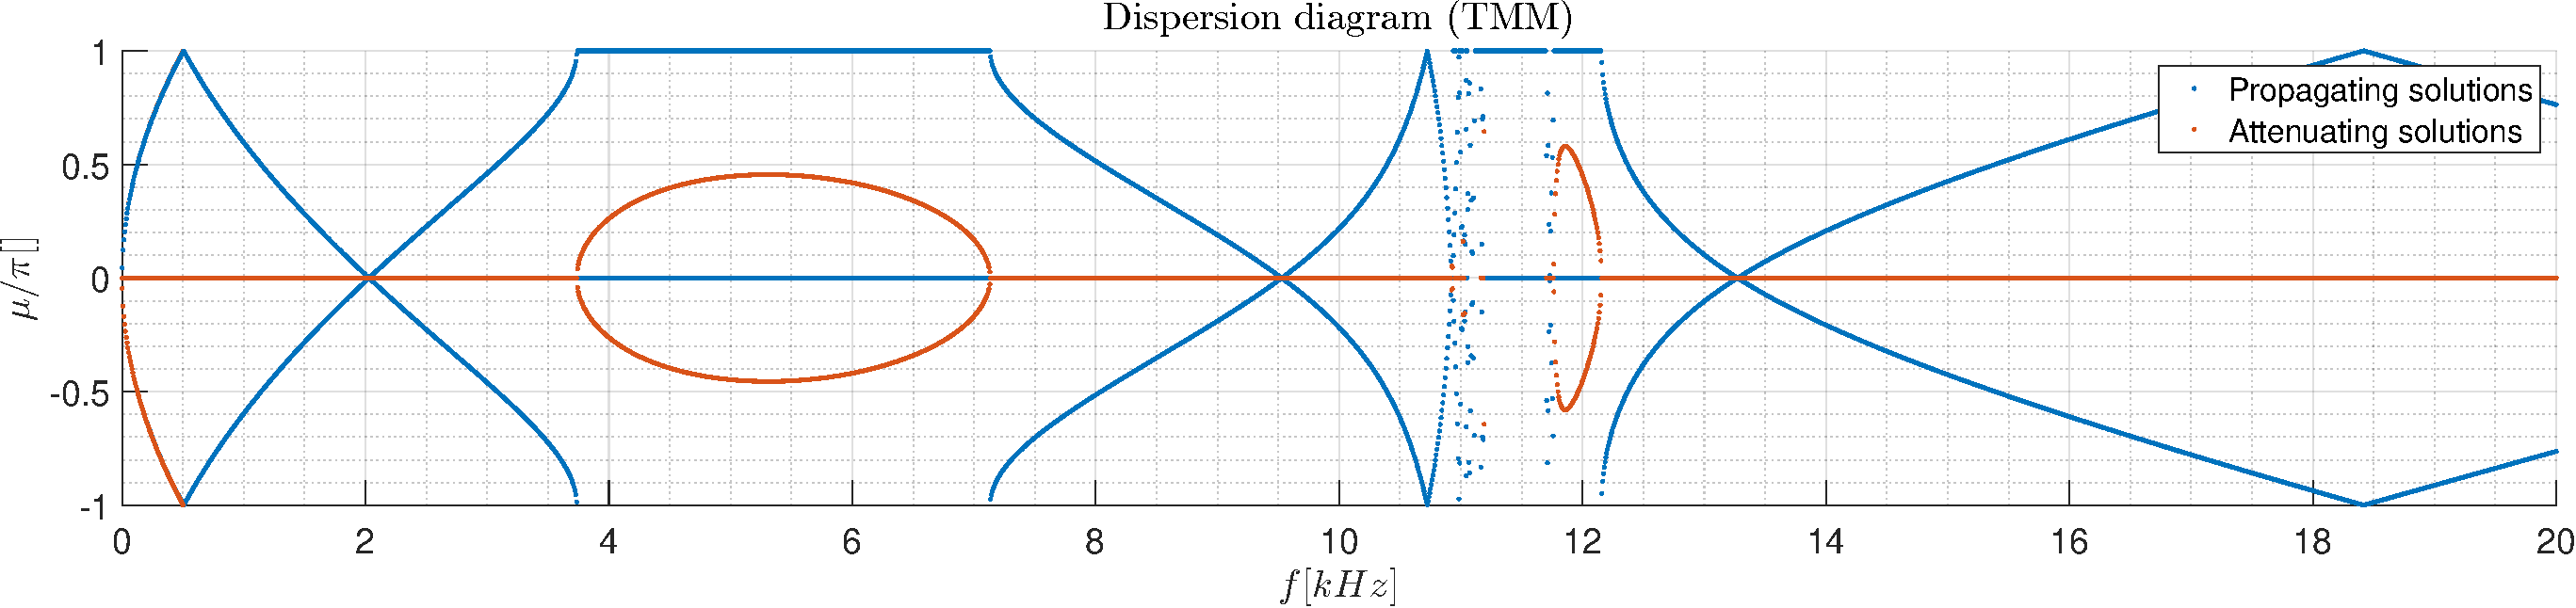
\includegraphics[width=\textwidth]{./img/MATLAB/TMM_ON-ON-ON_RLC_R50_L0.03_CInf.pdf}
            \caption{RLC shunt circuit with $R = 50 \Omega$, $L = 0.03 H$, and $C = \infty F$.}

        \end{figure}

    }

    \only<3-4>{

        \begin{figure}[H]
            \centering
            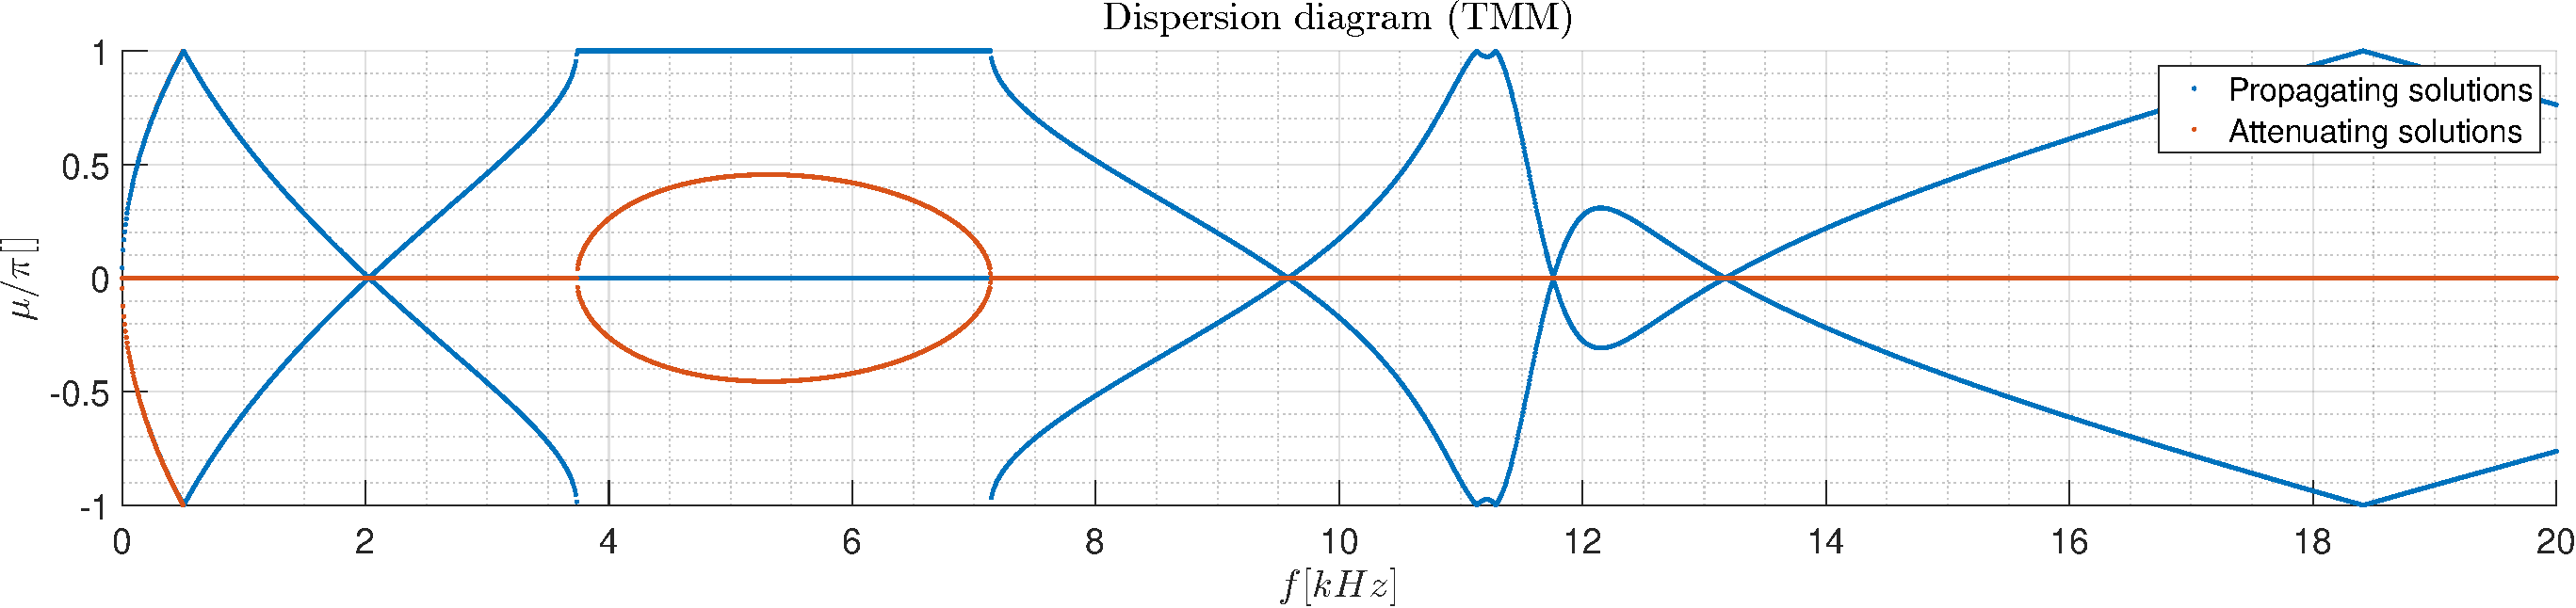
\includegraphics[width=\textwidth]{./img/MATLAB/TMM_ON-ON-ON_RLC_R200_L0.03_CInf.pdf}
            \caption{RLC shunt circuit with $R = 200 \Omega$, $L = 0.03 H$, and $C = \infty F$.}

        \end{figure}

    }

    \only<4->{

        \begin{figure}[H]
            \centering
            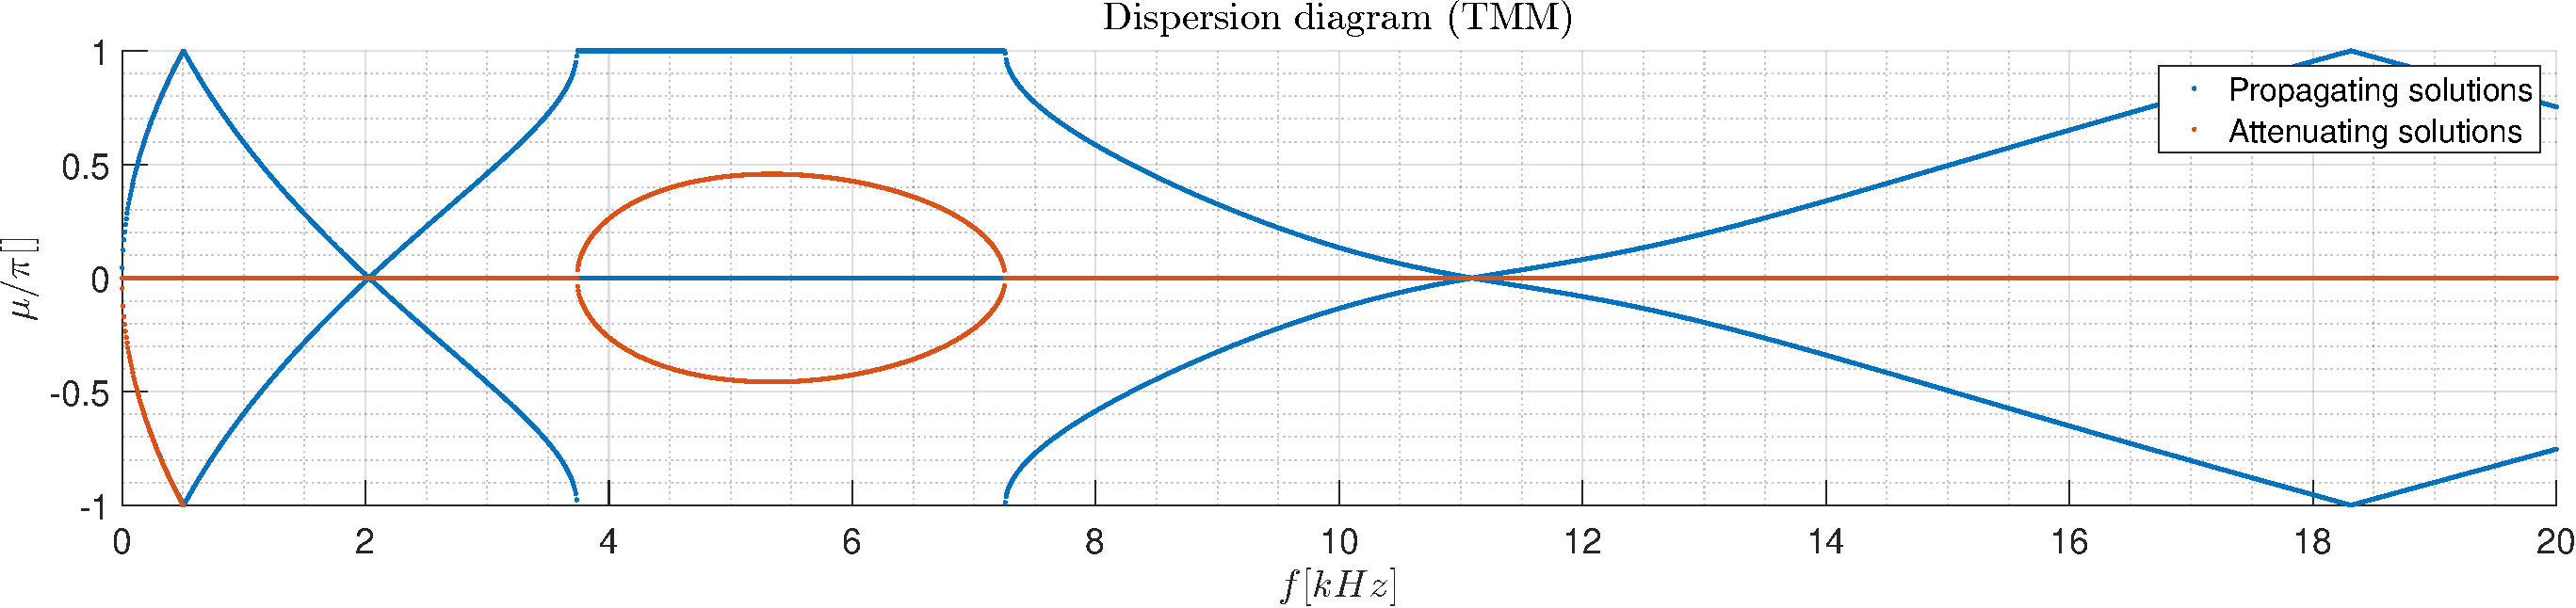
\includegraphics[width=\textwidth]{./img/MATLAB/TMM_ON-ON-ON_RLC_R1000_L0.03_CInf.pdf}
            \caption{RLC shunt circuit with $R = 1000 \Omega$, $L = 0.03 H$, and $C = \infty F$.}
        \end{figure}

    }

\end{frame}



\begin{frame}{$RC_N$ shunt circuit}

    \begin{figure}[H]
        \centering
        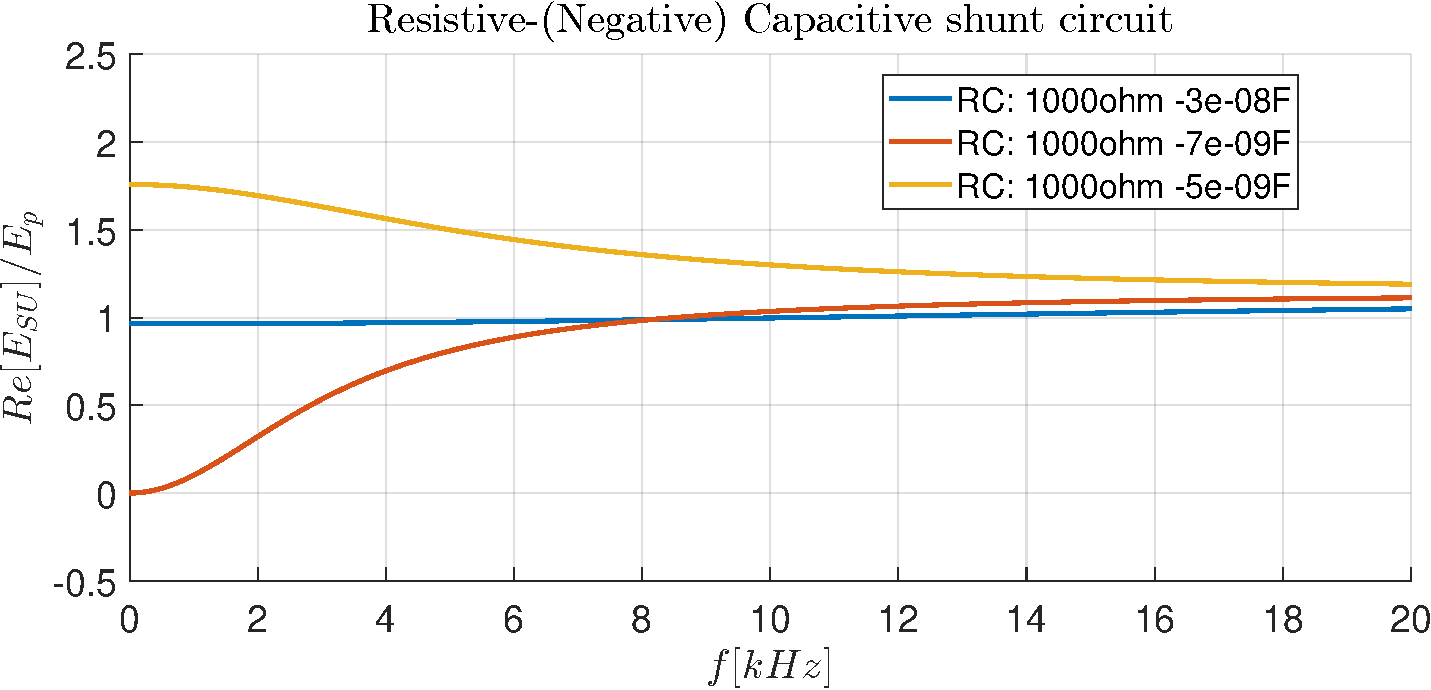
\includegraphics[width=0.6\textwidth]{./img/MATLAB/Y_SU_Resistive-(Negative) Capacitive shunt circuit.pdf}
        \caption{Analysis of $Y^{SU}$ for the resistive-(negative) capacitive shunt circuit.}
    \end{figure}

    In case of $RC_N$ shunt circuit, mechanical admittance of the piezoelectric patches is given by:

    \begin{equation}
        Y^{SU} = Y_1^D \left( 1 - \frac{k_{31}^2}{1 - C_p^S \frac{1}{C_N} - s C_p^S R} \right)
    \end{equation}

    The capacitative element has similar effects as the inductive one, with the ability to shift the band-gap toward lower or higher frequencies depending on the sign of $1 - C_p^S \frac{1}{C_N}$.

\end{frame}



\begin{frame}{$RC_N$ shunt circuit}

    \only<1-2>{

        \begin{figure}[H]
            \centering
            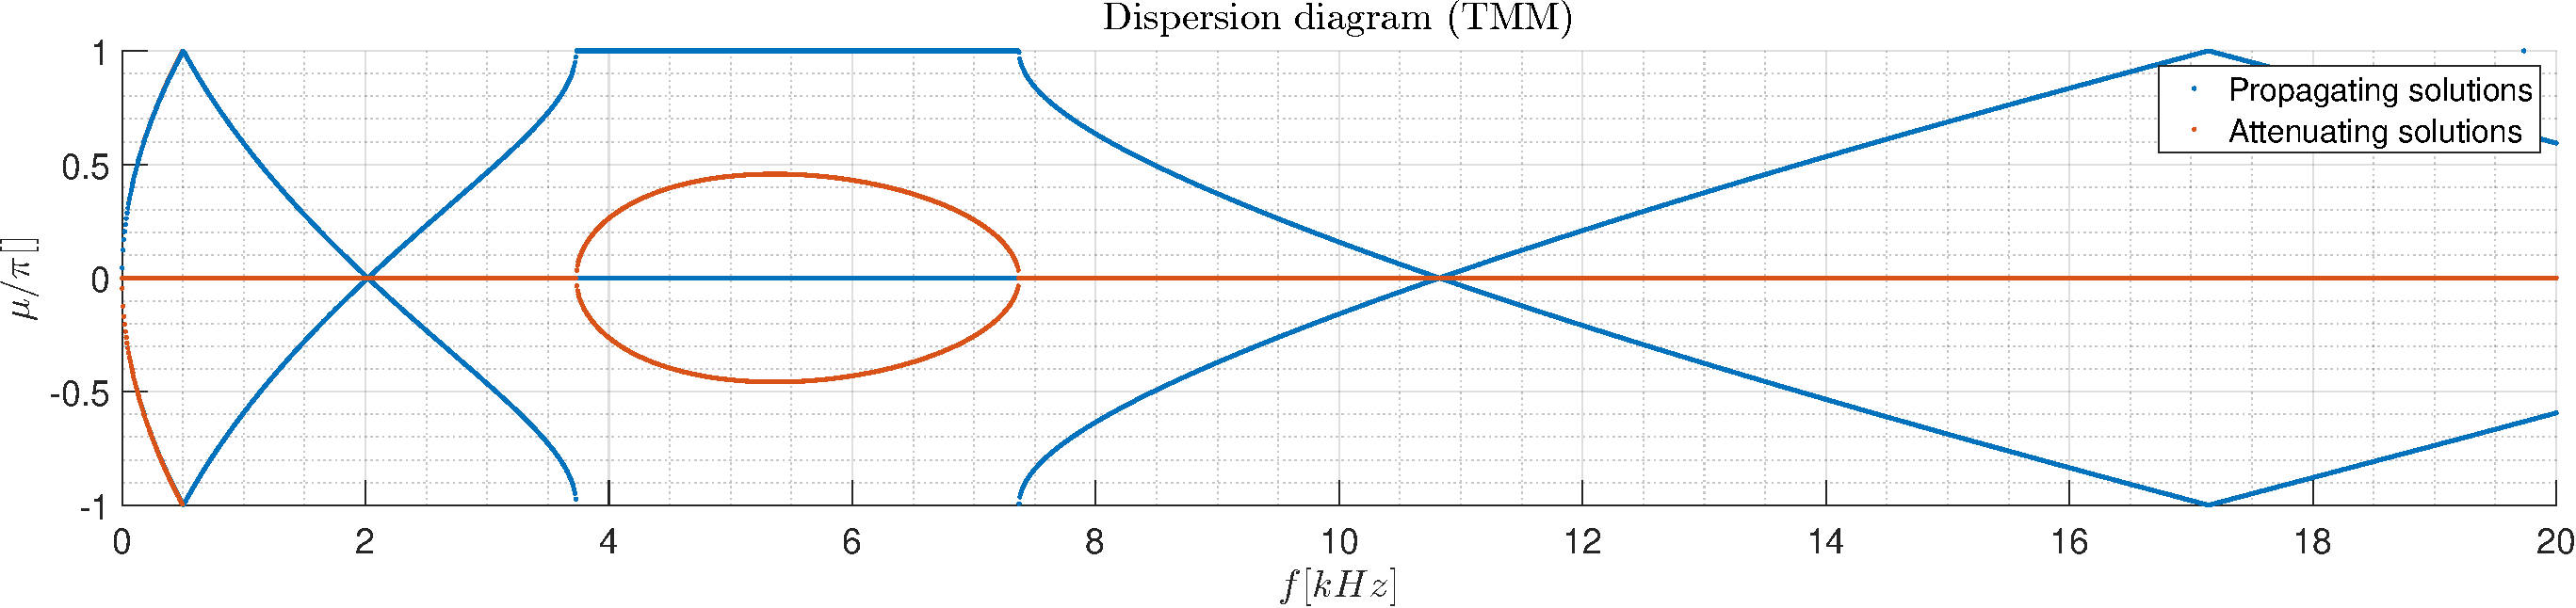
\includegraphics[width=\textwidth]{./img/MATLAB/TMM_ON-ON-ON_RLC_R1000_L0_C-3e-08.pdf}
            \caption{RLC shunt circuit with $R = 1000 \Omega$, $L = 0 H$, and $C = -30 nF$.}
        \end{figure}

    }

    \only<2-3>{

        \begin{figure}[H]
            \centering
            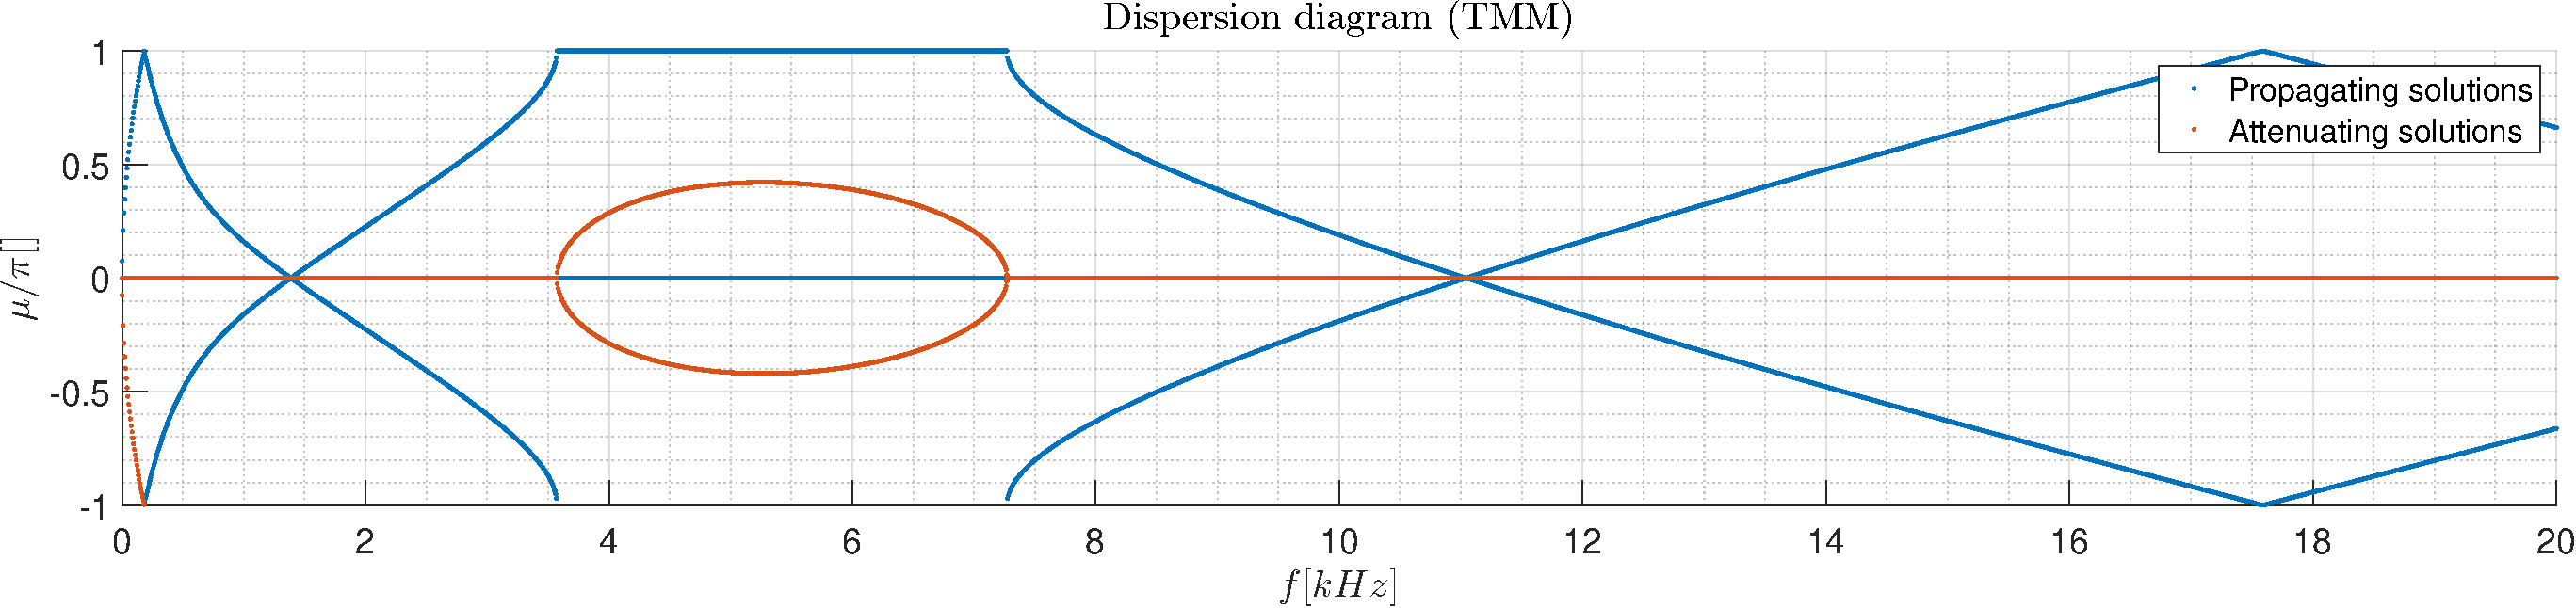
\includegraphics[width=\textwidth]{./img/MATLAB/TMM_ON-ON-ON_RLC_R1000_L0_C-7e-09.pdf}
            \caption{RLC shunt circuit with $R = 1000 \Omega$, $L = 0 H$, and $C = -7 nF$.}
        \end{figure}

    }

    \only<3->{

        \begin{figure}[H]
            \centering
            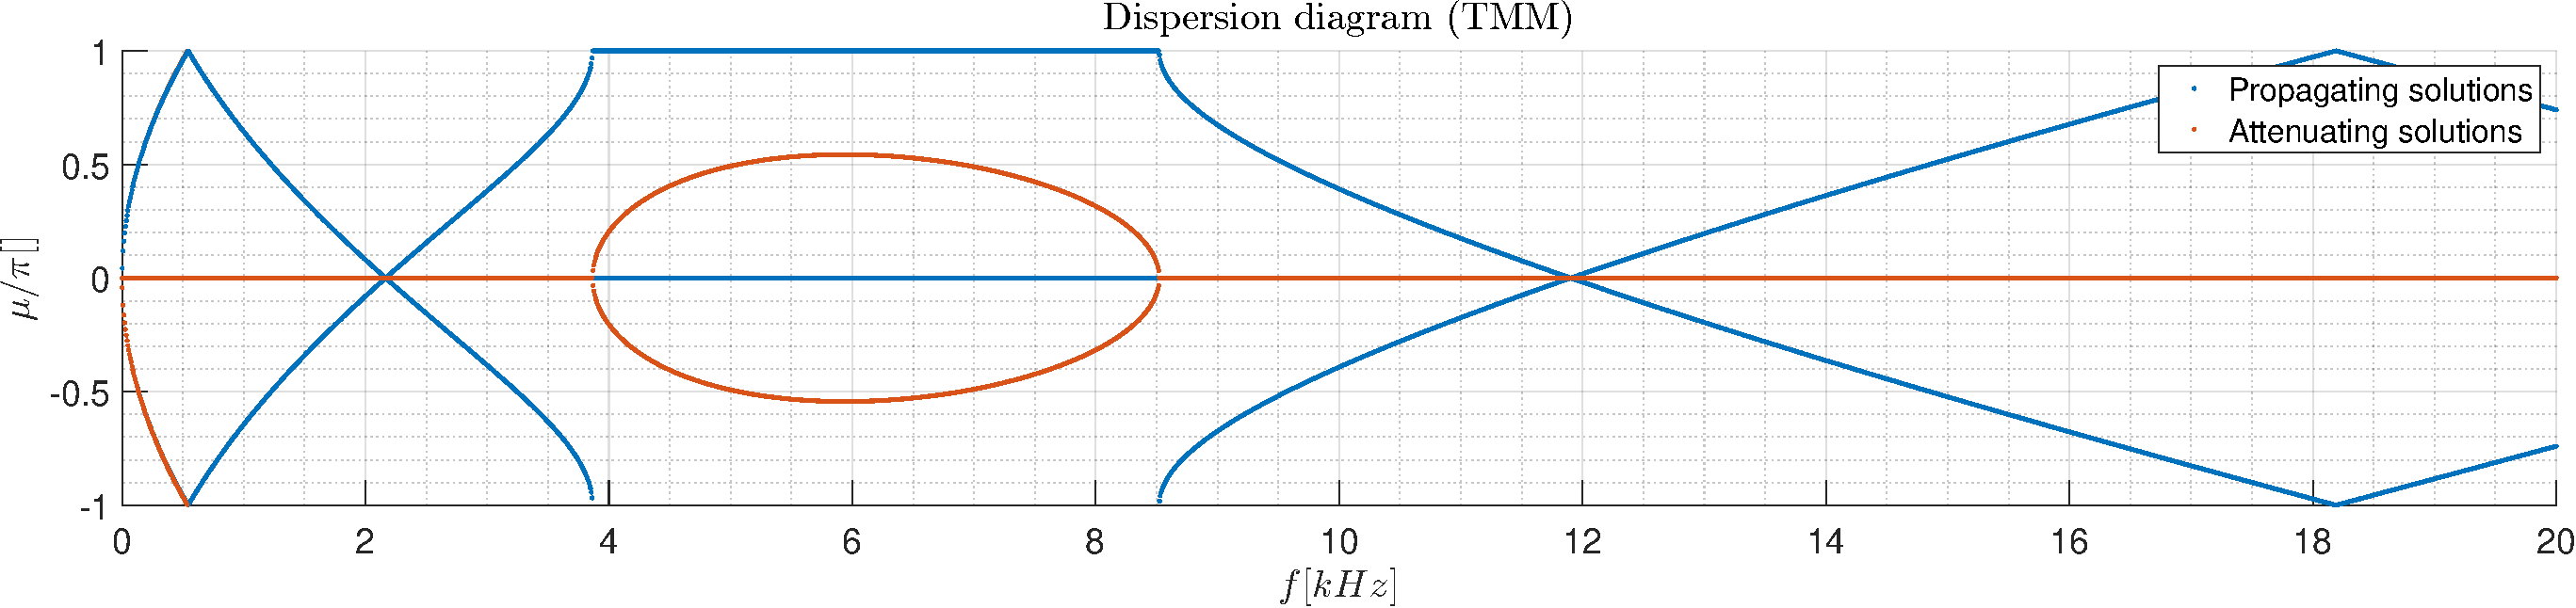
\includegraphics[width=\textwidth]{./img/MATLAB/TMM_ON-ON-ON_RLC_R1000_L0_C-5e-09.pdf}
            \caption{RLC shunt circuit with $R = 1000 \Omega$, $L = 0 H$, and $C = -5 nF$.}
        \end{figure}

    }

\end{frame}
